% Font options: 10pm, 11pt, 12pt
% Align headings left instead of center: nocenter
\documentclass[xcolor=x11names,compress]{beamer}\usepackage[]{graphicx}\usepackage[]{color}
%% maxwidth is the original width if it is less than linewidth
%% otherwise use linewidth (to make sure the graphics do not exceed the margin)
\makeatletter
\def\maxwidth{ %
  \ifdim\Gin@nat@width>\linewidth
    \linewidth
  \else
    \Gin@nat@width
  \fi
}
\makeatother

\definecolor{fgcolor}{rgb}{0.345, 0.345, 0.345}
\newcommand{\hlnum}[1]{\textcolor[rgb]{0.686,0.059,0.569}{#1}}%
\newcommand{\hlstr}[1]{\textcolor[rgb]{0.192,0.494,0.8}{#1}}%
\newcommand{\hlcom}[1]{\textcolor[rgb]{0.678,0.584,0.686}{\textit{#1}}}%
\newcommand{\hlopt}[1]{\textcolor[rgb]{0,0,0}{#1}}%
\newcommand{\hlstd}[1]{\textcolor[rgb]{0.345,0.345,0.345}{#1}}%
\newcommand{\hlkwa}[1]{\textcolor[rgb]{0.161,0.373,0.58}{\textbf{#1}}}%
\newcommand{\hlkwb}[1]{\textcolor[rgb]{0.69,0.353,0.396}{#1}}%
\newcommand{\hlkwc}[1]{\textcolor[rgb]{0.333,0.667,0.333}{#1}}%
\newcommand{\hlkwd}[1]{\textcolor[rgb]{0.737,0.353,0.396}{\textbf{#1}}}%
\let\hlipl\hlkwb

\usepackage{framed}
\makeatletter
\newenvironment{kframe}{%
 \def\at@end@of@kframe{}%
 \ifinner\ifhmode%
  \def\at@end@of@kframe{\end{minipage}}%
  \begin{minipage}{\columnwidth}%
 \fi\fi%
 \def\FrameCommand##1{\hskip\@totalleftmargin \hskip-\fboxsep
 \colorbox{shadecolor}{##1}\hskip-\fboxsep
     % There is no \\@totalrightmargin, so:
     \hskip-\linewidth \hskip-\@totalleftmargin \hskip\columnwidth}%
 \MakeFramed {\advance\hsize-\width
   \@totalleftmargin\z@ \linewidth\hsize
   \@setminipage}}%
 {\par\unskip\endMakeFramed%
 \at@end@of@kframe}
\makeatother

\definecolor{shadecolor}{rgb}{.97, .97, .97}
\definecolor{messagecolor}{rgb}{0, 0, 0}
\definecolor{warningcolor}{rgb}{1, 0, 1}
\definecolor{errorcolor}{rgb}{1, 0, 0}
\newenvironment{knitrout}{}{} % an empty environment to be redefined in TeX

\usepackage{alltt}
%\documentclass[xcolor=x11names,compress,handout]{beamer}
\usepackage[]{graphicx}
\usepackage[]{color}
\usepackage{booktabs}
\usepackage{hyperref}
\usepackage{tikz}
\usepackage{multirow}
\usepackage{dcolumn}
\usepackage{bigstrut}
\usepackage{amsmath} 
\usepackage{xcolor,colortbl}
\usepackage{amssymb}
\usepackage{multicol}
%\newcommand{\done}{\cellcolor{teal}#1}

%% Beamer Layout %%%%%%%%%%%%%%%%%%%%%%%%%%%%%%%%%%
\useoutertheme[subsection=false,shadow]{miniframes}
\useinnertheme{default}
\usefonttheme{serif}
\usepackage{Arev}
\usepackage{pdfpages}

\setbeamerfont{title like}{shape=\scshape}
\setbeamerfont{frametitle}{shape=\scshape, size=\normalsize}

\definecolor{dkblue}{RGB}{0,0,102}

\setbeamercolor*{lower separation line head}{bg=dkblue} 
\setbeamercolor*{normal text}{fg=black,bg=white} 
\setbeamercolor*{alerted text}{fg=red} 
\setbeamercolor*{example text}{fg=black} 
\setbeamercolor*{structure}{fg=black} 
 
\setbeamercolor*{palette tertiary}{fg=black,bg=black!10} 
\setbeamercolor*{palette quaternary}{fg=black,bg=black!10} 

\renewcommand{\(}{\begin{columns}}
\renewcommand{\)}{\end{columns}}
\newcommand{\<}[1]{\begin{column}{#1}}
\renewcommand{\>}{\end{column}}

\AtBeginSection{\frame{\sectionpage}}
\usepackage{xcolor}
\hypersetup{
    colorlinks,
    linkcolor={red!50!black},
    citecolor={blue!50!black},
    urlcolor={blue!80!black}
}

\setbeamertemplate{navigation symbols}{} 
\setbeamertemplate{footline}[frame number]
\setbeamertemplate{caption}{\raggedright\insertcaption\par}

\setbeamersize{text margin left=5pt,text margin right=5pt}

%%%%%%%%%%%%%%%%%%%%%%%%%%%%%%%%%%%%%%%%%%%%%%%%%%


\title{FLS 6441 - Methods III: Explanation and Causation}
\subtitle{Week 11 - Comparative Case Studies \& Process Tracing}
\author{Jonathan Phillips}
\date{June 2019}
\IfFileExists{upquote.sty}{\usepackage{upquote}}{}
\begin{document}




\frame{\titlepage}

\begin{frame}
\frametitle{Classification of Research Designs}
\footnotesize
\begin{table}[htbp]
  \centering
  \scalebox{0.7}{
    \begin{tabular}{|p{2.2cm}|p{5cm}|c|c|}
    \hline
          &       & \multicolumn{1}{p{2.4cm}|}{\textbf{Independence of Treatment Assignment}} & \multicolumn{1}{p{3cm}|}{\textbf{Researcher Controls Treatment Assignment?}} \bigstrut\\
    \hline
    \multicolumn{1}{|p{2.9cm}|}{\multirow{2}[4]{2.9cm}{\textbf{Controlled Experiments}}} & Field Experiments & \checkmark      & \checkmark  \bigstrut\\
\cline{2-4}          & Survey and Lab Experiments &  \checkmark     & \checkmark \bigstrut\\
    \hline
          &       &       &  \bigstrut\\
    \hline
    \multicolumn{1}{|p{2.9cm}|}{\multirow{3}[6]{2.9cm}{\textbf{Natural Experiments}}} & Natural Experiments &  \checkmark     &  \bigstrut\\
\cline{2-4}          & Instrumental Variables & \checkmark      &  \bigstrut\\
\cline{2-4}          & Discontinuities & \checkmark      &  \bigstrut\\
    \hline
          &       &       &  \bigstrut\\
    \hline
    \multicolumn{1}{|p{2.9cm}|}{\multirow{4}[8]{2.9cm}{\textbf{Observational Studies}}} & Difference-in-Differences &       &  \bigstrut\\
\cline{2-4}          & Controlling for Confounding &       &  \bigstrut\\
\cline{2-4}          & Matching &       &  \bigstrut\\
\cline{2-4}          & Comparative Cases and Process Tracing &       &  \bigstrut\\
    \hline
    \end{tabular}}%
  \label{tab:addlabel}%
\end{table}%
\normalsize
\end{frame}

\section{Comparative Case Studies} 

\begin{frame}
\frametitle{Comparative Case Studies}
\begin{itemize}
\item Necessary when there are few measurable cases of our treatment/outcome
\pause
\item \textbf{Exactly} the same causal inference logic as Large-N
\pause
\item We need counterfactuals to estimate treatment effects: \textbf{Comparative} Cases
\end{itemize}
\end{frame}

\begin{frame}
\frametitle{Comparative Case Studies}
\begin{itemize}
\item Why can't we achieve causal inference from single case studies?
\pause
\item If we have only one 'treated' observation, we \textit{cannot} know what would have happened in the absence of treatment
\begin{itemize}
\item Exactly the same outcome could have occurred
\end{itemize}
\pause
\item These case studies can help \textit{generate} hypotheses...
\pause
\item ...And they can maybe weaken a theory... eg. if the outcome is absent with treatment
\pause
\item But they cannot \textbf{confirm} a theory
\pause
\item We need variation in the dependent variable if we are to \textit{explain} it
\pause
\item Common error: "research that tries to explain the outbreak of war with studies only of wars" (KKV)
\end{itemize}
\end{frame}

\begin{frame}
\frametitle{Comparative Case Studies}
\begin{itemize}
\item In a small-N study, what causal inference technique is most useful?
\pause
\begin{itemize}
\item \textbf{Natural experiments:} Possible, but rare
\pause
\item \textbf{Diff-in-diff:} Maybe if we have time-series data
\pause
\item \textbf{Controlling:} Not enough observations
\pause
\item \textbf{Matching:} More useful
\end{itemize}
\end{itemize}
\end{frame}

\begin{frame}
\frametitle{Comparative Case Studies}
\begin{itemize}
\item Matching is the \textbf{'Comparative Method'}
\begin{itemize}
\item Don't look at the outcome variable
\pause
\item Split the sample on a single treatment variable
\pause
\item Balance on confounders through careful case selection - remove unmatched cases
\pause
\item We can't match on everything, so focus on getting balance on \textbf{key confounders/alternative theories}
\pause
\end{itemize}
\item \textbf{Our Large-N dataset after matching might look very similar to comparative case studies}
\end{itemize}
\end{frame}

\begin{frame}
\frametitle{Comparative Case Studies}
\begin{itemize}
\item Does Development cause Democracy?
\pause
\item We want cases which vary in level of development
\pause
\item But are identical in all other ways \pause \textbf{Impossible!}
\end{itemize}
\end{frame}

\begin{frame}
\frametitle{Comparative Case Studies}
\begin{itemize}
\item Does Development cause Democracy?
\item We want cases which vary in level of development
\item But are identical in the other variables theory suggests might be confounders \pause \textbf{Possible!}
\begin{itemize}
\item Or at least those variables which suggest the treated case would be \textit{less} democratic
\end{itemize}
\pause
\item Alternative Theories of Democratization:
\begin{enumerate}
\item Geography
\pause
\item Religion/culture
\pause
\item Inequality
\pause
\item Slow economic growth
\end{enumerate}
\end{itemize}
\end{frame}

\begin{frame}
\frametitle{Comparative Case Studies}
\begin{table}[htbp]
  \centering
  \caption{Does Development cause Democracy?}
    \begin{tabular}{|r|l|c|c|}
    \hline
          & Variable & \multicolumn{1}{l|}{Case A} & \multicolumn{1}{l|}{Case B} \bigstrut\\
    \hline
    \multicolumn{1}{|l|}{Outcome} & Democracy & ?     & ? \bigstrut\\
    \hline
    \multicolumn{1}{|l|}{Treatment} & Development & Low   & High \bigstrut\\
    \hline
    \multicolumn{1}{|l|}{Controls} & Religion & Christian & Christian \bigstrut\\
    \hline
          & Continent & Europe & Europe \bigstrut\\
    \hline
          & Inequality & 0.45  & 0.44 \bigstrut\\
    \hline
          & Economic growth & 1.2\% & 5\% \bigstrut\\
    \hline
          & National dish & Pasta & Corn \bigstrut\\
    \hline
          & Length of Railways & 400km & 120km \bigstrut\\
    \hline
    \end{tabular}%
  \label{tab:addlabel}%
\end{table}%
\end{frame}

\begin{frame}
\frametitle{Comparative Case Studies}
\begin{itemize}
\item Similarities with Large-N:
\pause
\begin{itemize}
\item Same challenges to inference: confounding, selection, reverse causation
\pause
\item Same assumptions required: SUTVA, Balance on all confounders
\pause
\end{itemize}
\item Differences with Large-N:
\begin{itemize}
\item Harder to balance confounders: More variables than cases!
\pause
\item Fewer comparisons: No uncertainty measure or confidence intervals. What's our standard of evidence?
\pause
\begin{itemize}
\item p-values aren't the only source of credibility (Slater and Ziblatt 2013)
\end{itemize}
\pause
\item Statistical Inference: Non-random case-selection, so generalization is harder
\end{itemize}
\end{itemize}
\end{frame}

\begin{frame}
\frametitle{Comparative Case Studies}
\begin{itemize}
\item Case Selection:
\pause
\item Two distinct considerations:
\pause
\begin{enumerate}
\item \textbf{Causal Inference} (internal validity) - can our cases tell us with confidence that $D$ causes $Y$?
\pause
\item \textbf{Statistical Inference} (external validity) - How much can we generalize about this causal effect to a broader population?
\pause
\end{enumerate}
\item Ideally we want both: Control and representative variation
\pause
\begin{itemize}
\item Our goal is not to explain why outcome $Y$ happened in one case, but why it happens generally
\end{itemize}
\end{itemize}
\end{frame}

\begin{frame}
\frametitle{Comparative Case Studies}
\begin{itemize}
\item Case Selection:
\pause
\begin{itemize}
\item Random sampling is fine! It directly helps us generalize
\pause
\item And it helps us avoid researcher bias
\pause
\item But:
\pause
\begin{itemize}
\item Randomization does not guarantee balance on confounders in small samples
\pause
\item Randomized sampling is not the same as randomized treatment
\end{itemize}
\item Probably easier to 'block' on key confounders and impose variation in treatment - purposive sampling
\end{itemize}
\end{itemize}
\end{frame}

\begin{frame}
\frametitle{Comparative Case Studies}
\begin{itemize}
\item Can we really ignore the outcome variable??
\pause
\begin{itemize}
\item \textbf{DO NOT} select cases by the value of the outcome (Geddes)
\begin{itemize}
\pause
\item If we only study success cases, we don't know the outcome under control
\pause
\item The 'treatment' may also have been present in the 'control' cases
\pause
\item We want to explain interesting things, so we often pick 'extreme' cases, but the extremeness might reflect confounders, not the treatment
\end{itemize}
\pause
\item But: If we select cases explicitly for a \textit{range} of values of the outcome, that's better
\end{itemize}
\end{itemize}
\end{frame}

\begin{frame}
\frametitle{Comparative Case Studies}
\begin{itemize}
\item Generalizability:
\pause
\begin{itemize}
\item Depends on our cases being representative
\pause
\item If we want to compare men's and women's running speeds, \textbf{DO NOT} pick Usain Bolt and Florence Griffith-Joyner
\pause
\item Pick units with 'median' values - or a range of values - on the confounding and outcome variables
\pause
\item At the same time as balancing confounders - hard!
\end{itemize}
\end{itemize}
\end{frame}

\begin{frame}
\frametitle{Comparative Case Studies}
\begin{itemize}
\item \textbf{Most similar cases:} Same covariates, different treatment value
\pause
\item BUT If there are many sets of 'most similar' paired cases, which should we pick?
\pause
\begin{itemize}
\item \textbf{Typical cases:} Most representative paired cases on covariates, eg. Levitsky and Way
\pause
\item \textbf{Diverse cases:} Covering all values of treatment and covariates, eg. Slater
\pause
\item \textbf{Extreme cases:} Highest and lowest values of treatment, eg. Lieberman
\end{itemize}
\end{itemize}
\end{frame}

\begin{frame}
\frametitle{Comparative Case Studies}
\begin{itemize}
\item Methods for alternative objectives:
\pause
\begin{itemize}
\item \textbf{Deviant cases:} If you want to disprove a theory or generate a new hypothesis
\pause
\item \textbf{Most different cases:} When searching for a hypothesis to explain $Y$
\pause
\item \textbf{Influential cases:} How sensitive is our relationship to mismeasurement of a key case?
\end{itemize}
\end{itemize}
\end{frame}

\section{Mixed Methods}

\begin{frame}
\frametitle{Mixed Methods}
\begin{itemize}
\item How do we combine our earlier quantitative methods with comparative cases?
\pause
\item Three forms of mixed methods:
\pause
\begin{enumerate}
\item Large-N measurement supports \textbf{case selection} for Small-N analysis (Seawright and Gerring)
\pause
\item Comparative cases to identify explanation, then \textbf{tested for generalizability} in Large-N sample (Lieberman)
\pause
\item Large-N analysis to show \textbf{causal effect within-case}, then generalized using comparative case studies (Ziblatt and Slater)
\end{enumerate}
\end{itemize}
\end{frame}

\begin{frame}
\frametitle{Comparative Case Studies}
\begin{itemize}
\item Strategies for increasing the number of observations:
\pause
\begin{enumerate}
\item Additional measurable implications of the causal theory
\pause
\item Subnational units
\pause
\item Time-series
\pause
\item Alternative mesaures
\end{enumerate}
\end{itemize}
\end{frame}

\section{Process Tracing} 

\begin{frame}
\frametitle{Process Tracing}
\begin{itemize}
\item Can we learn anything with a single case study?
\pause
\item Yes: \textbf{Within-case analysis}
\pause
\item For testing \textbf{specific causal theories} - \textit{how} does $D$ affect $Y$?
\pause
\item Only possible if we can turn our \textbf{single case} into \textbf{multiple observations}
\pause
\item \textbf{Causal Process Observations:}
\begin{itemize}
\item Evidence must support or undermine a specific theory
\pause
\item What observable implications are there of theory A? How do they differ from the implications of theory B?
\pause
\item Is the evidence consistent with theory A? Or inconsistent with theory B?
\end{itemize}
\end{itemize}
\end{frame}

\begin{frame}
\frametitle{Process Tracing}
\begin{enumerate}
\item Identify all relevant theories to explain the outcome (treatment plus alternative theories)
\pause
\item For each theory what would the case look like if the theory was true?
\pause
\item Gather data from the case on each observable implication
\pause
\item Compare the data to each theory
\pause
\item Can we eliminate all other theories except our treatment?
\begin{itemize}
\item Sherlock Holmes' Method of Elimination
\end{itemize}
\end{enumerate}
\end{frame}

\begin{frame}
\frametitle{Process Tracing}
\begin{itemize}
\item We know the value of treatment and outcome for our case - and it fits our theory
\pause
\item But we don't have any counterfactual to compare against
\pause
\item The outcome could instead have been caused by a confounder
\end{itemize}
\begin{knitrout}
\definecolor{shadecolor}{rgb}{0.969, 0.969, 0.969}\color{fgcolor}
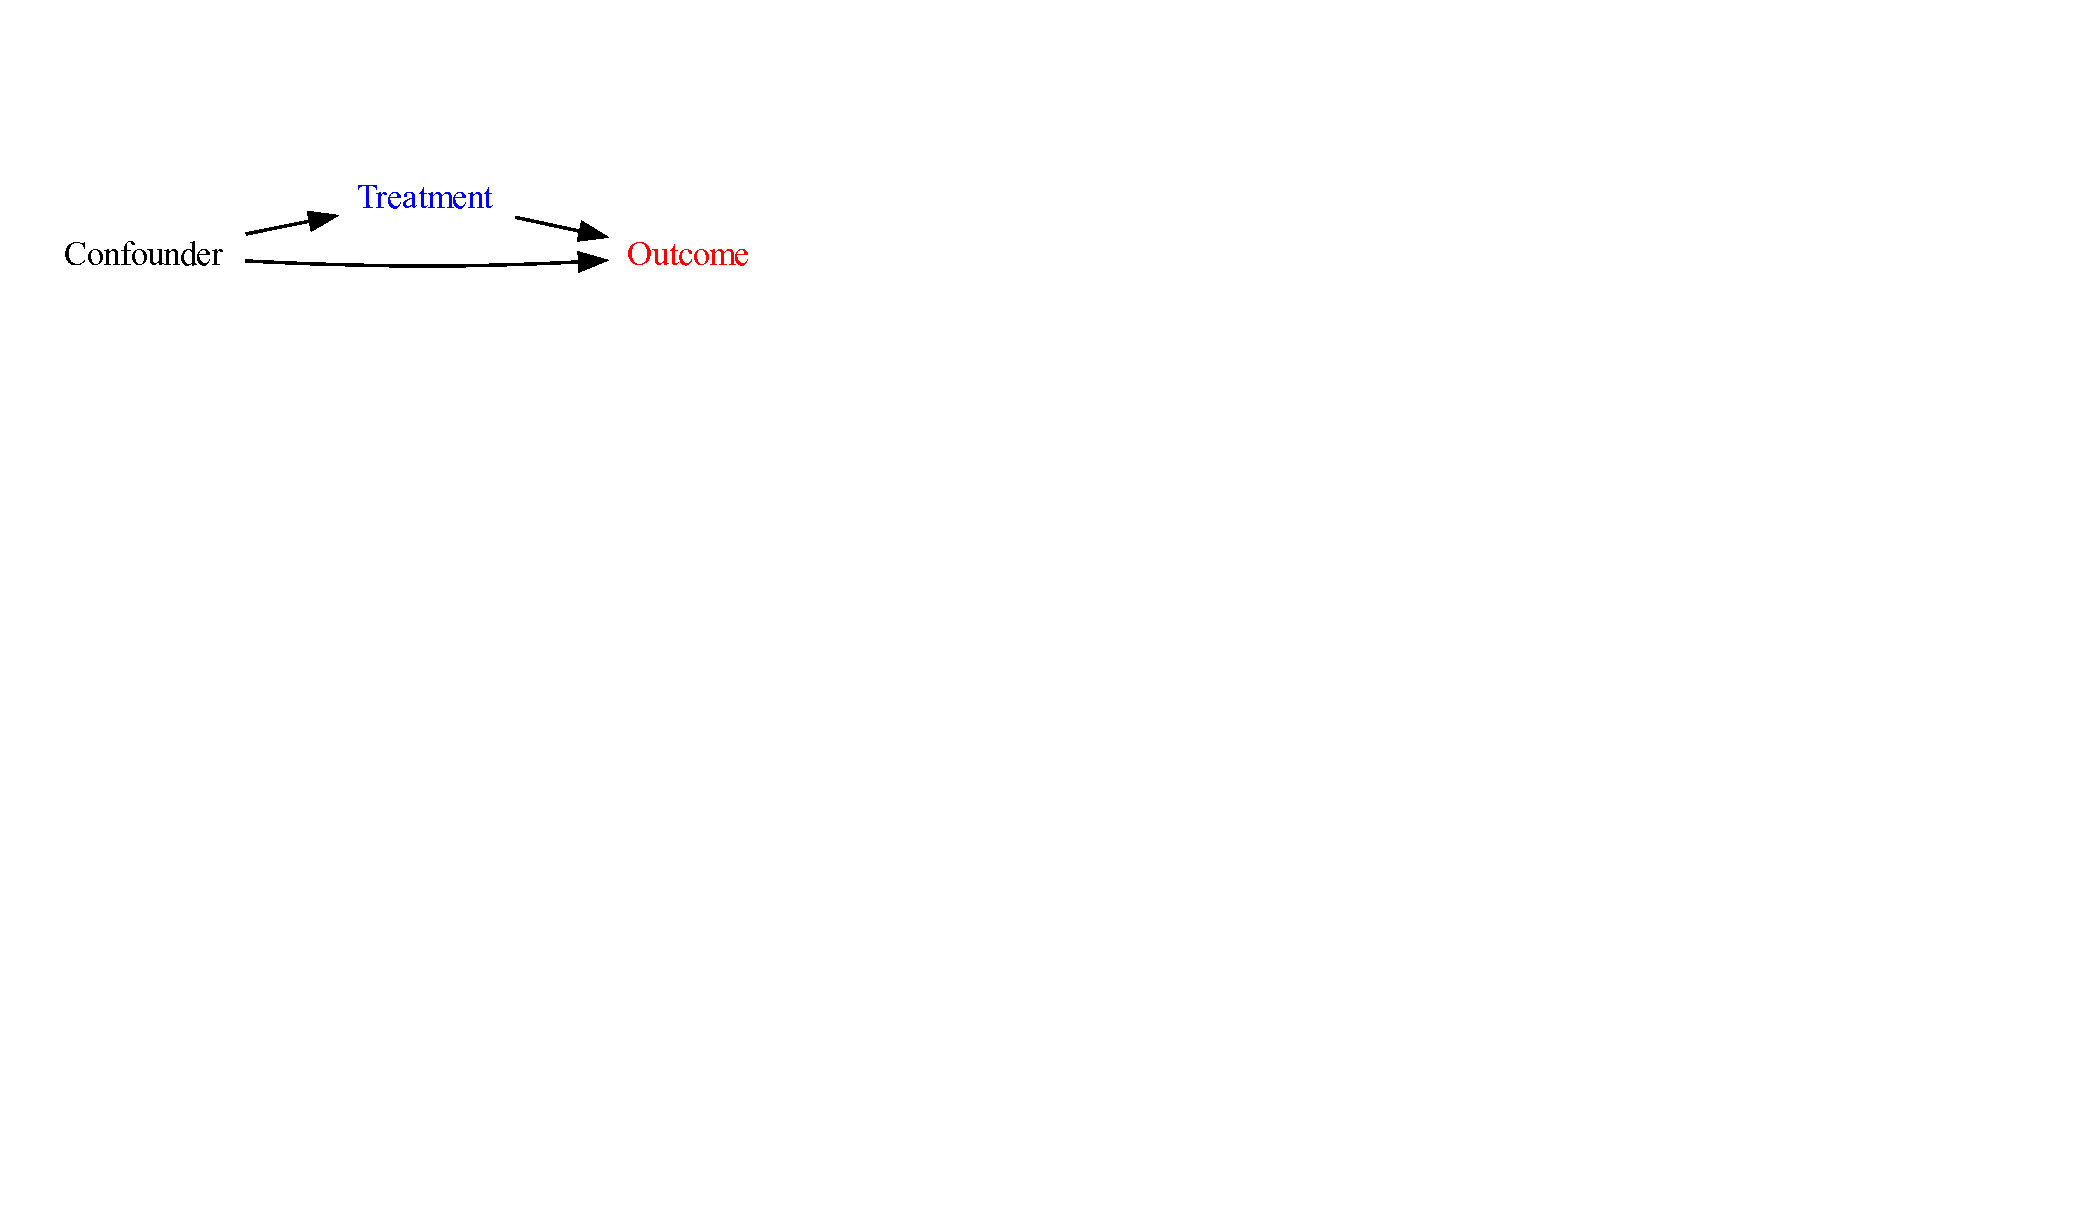
\includegraphics[width=1.8\linewidth]{figure/Dag1-1} 

\end{knitrout}
\end{frame}

\begin{frame}
\frametitle{Process Tracing}
\begin{itemize}
\item One way to support our theory is to test the mechanisms along the causal path of treatment:
\begin{itemize}
\item Evidence of M NOT occurring is proof Treatment did not have a causal effect
\item Evidence of M occurring is consistent with Treatment having a causal effect
\end{itemize}
\end{itemize}
\begin{knitrout}
\definecolor{shadecolor}{rgb}{0.969, 0.969, 0.969}\color{fgcolor}
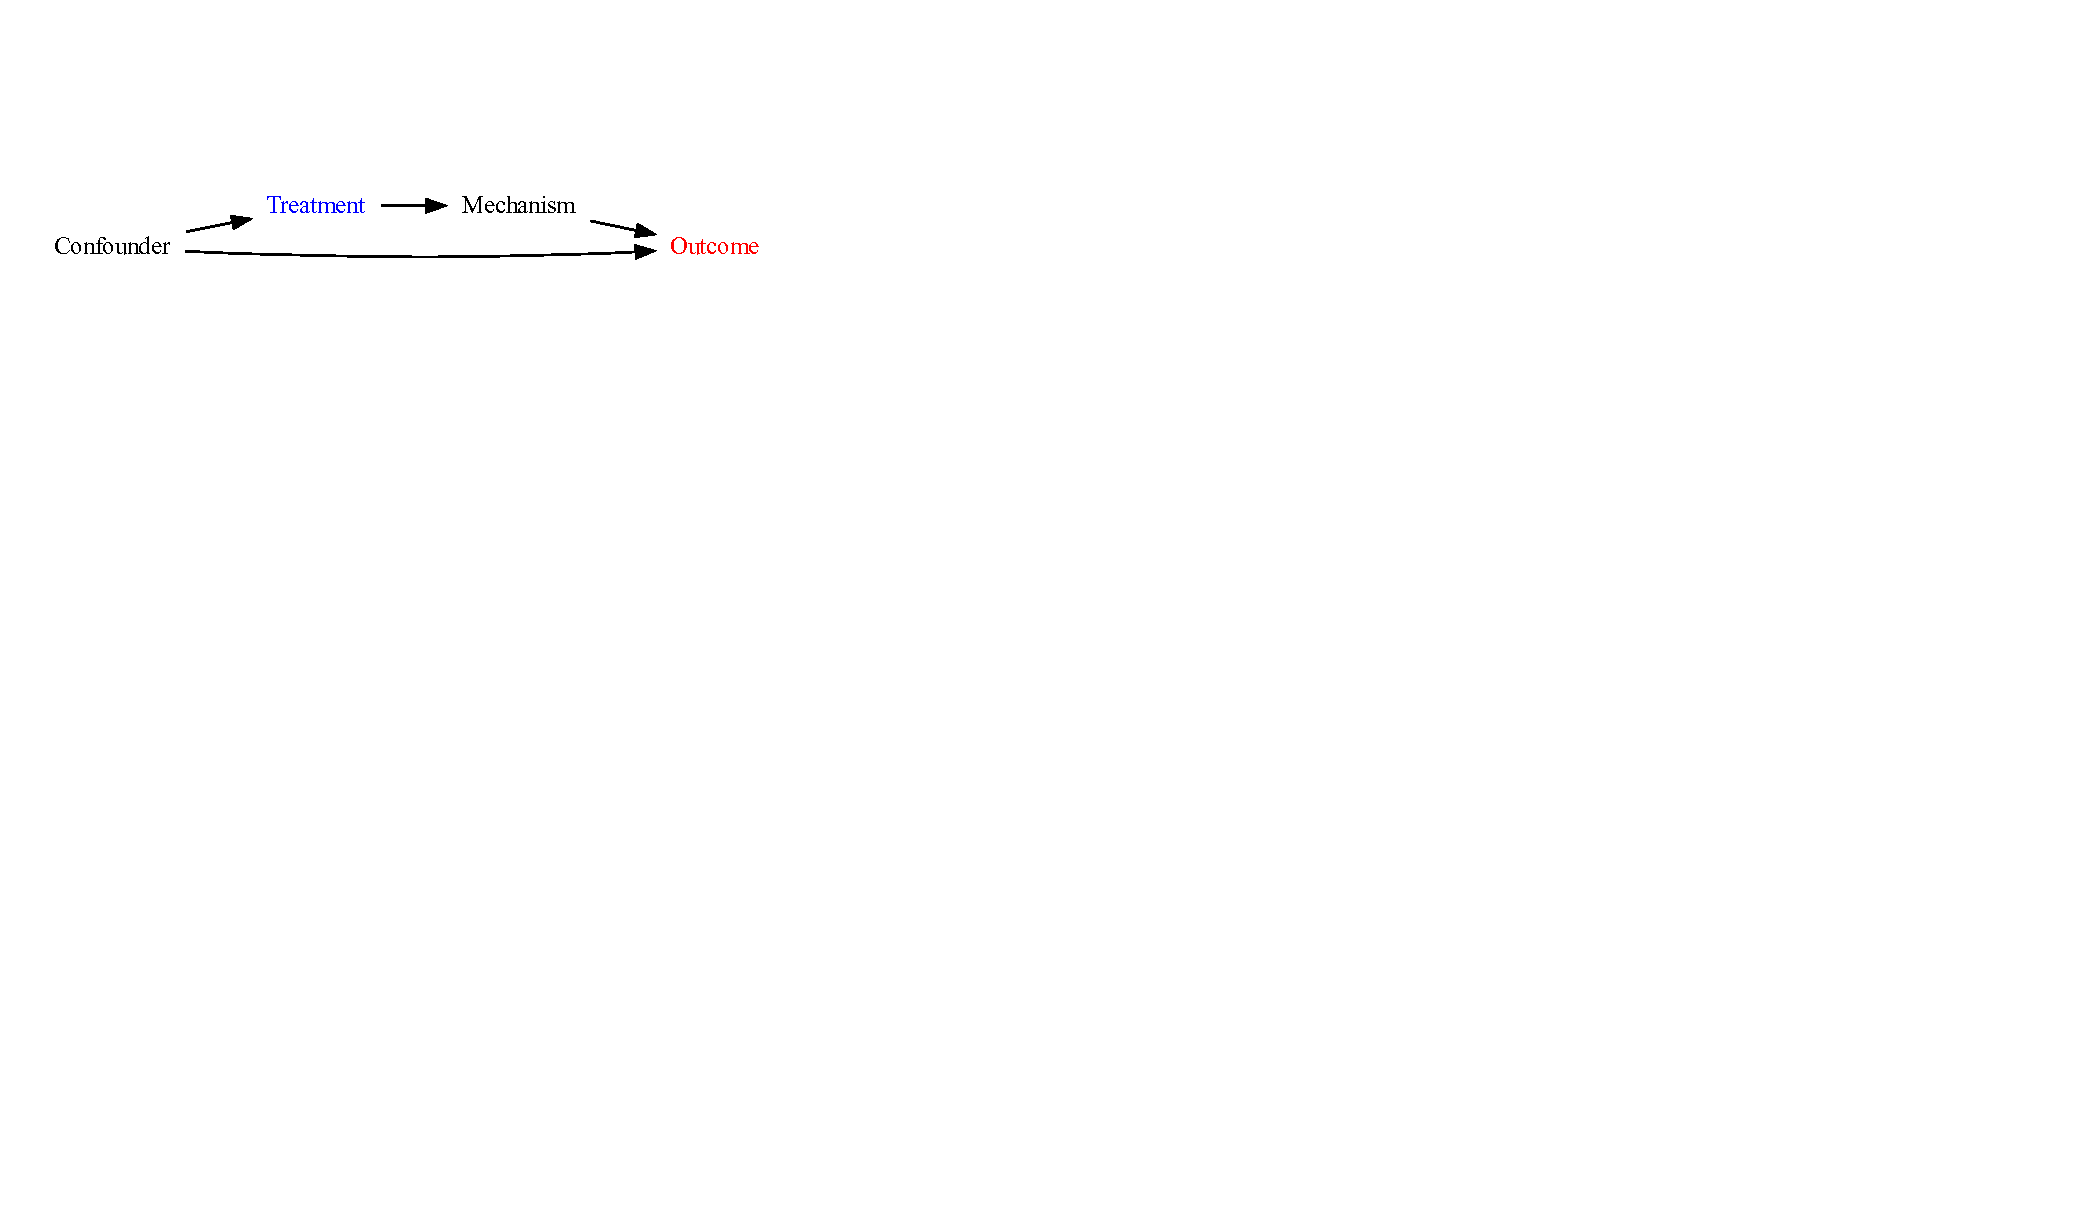
\includegraphics[width=1.8\linewidth]{figure/Dag2-1} 

\end{knitrout}
\end{frame}

\begin{frame}
\frametitle{Process Tracing}
\begin{itemize}
\item One way to support our theory is to test the mechanisms along the causal path of treatment:
\begin{itemize}
\item Evidence of M NOT occurring is proof Treatment did not have a causal effect
\item Evidence of M occurring is consistent with Treatment having a causal effect
\begin{itemize}
\item It could have been another confounder that also worked through that mechanism
\pause
\end{itemize}
\end{itemize}
\item This is a 'hoop' test
\end{itemize}
\begin{knitrout}
\definecolor{shadecolor}{rgb}{0.969, 0.969, 0.969}\color{fgcolor}
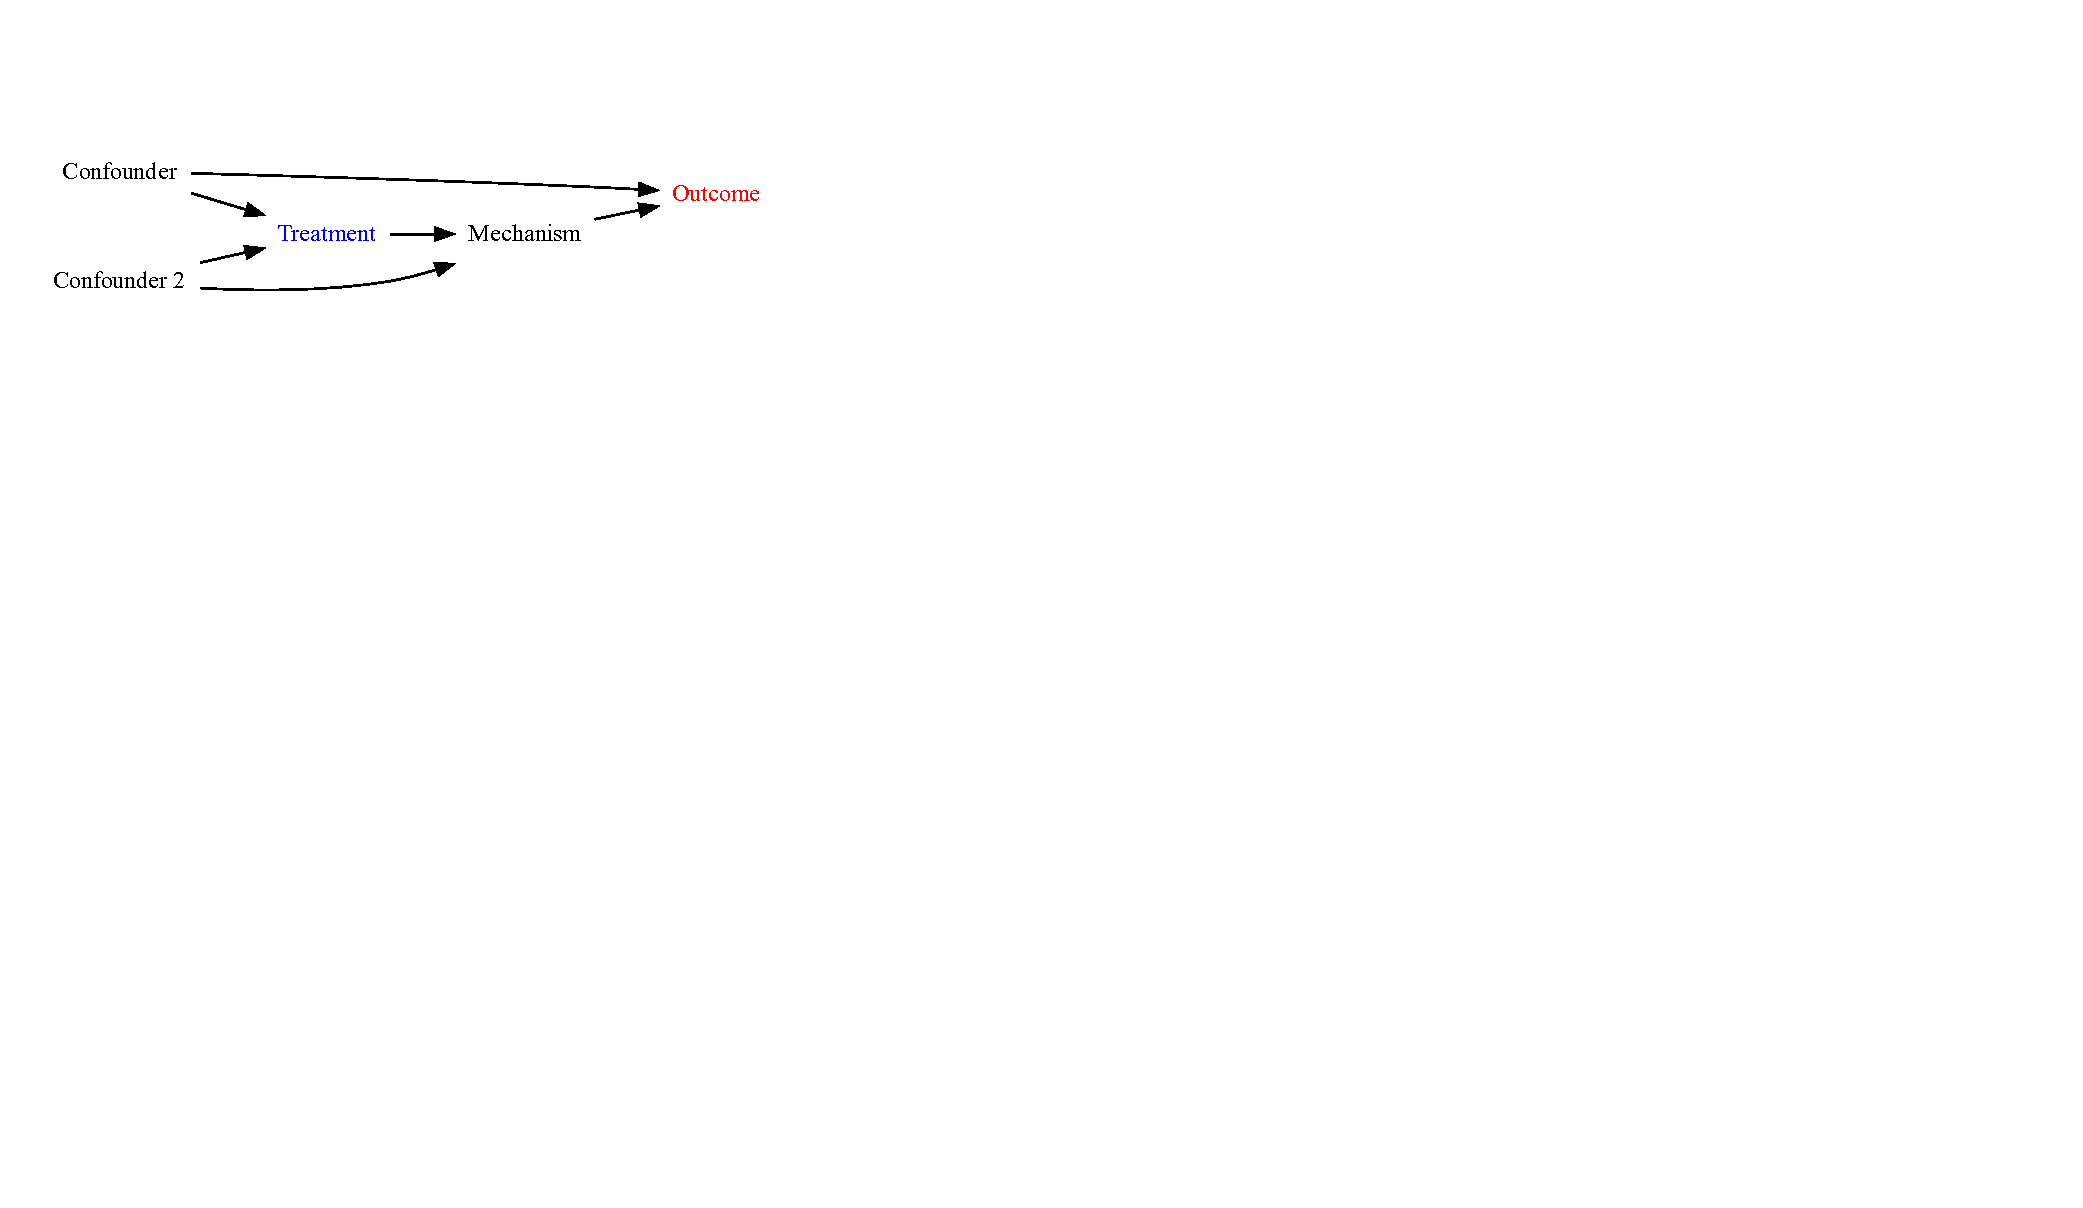
\includegraphics[width=1.8\linewidth]{figure/Dag3-1} 

\end{knitrout}
\end{frame}

\begin{frame}
\frametitle{Process Tracing}
\begin{itemize}
\item One way to support our theory is to test the mechanisms along the causal path of treatment:
\begin{itemize}
\item Evidence of M NOT occurring is proof Treatment did not have a causal effect
\item Evidence of M occurring is consistent with Treatment having a causal effect
\end{itemize}
\item If there are no other possible confounders consistent with this mechanism, this is a 'Smoking Gun' test
\end{itemize}
\begin{knitrout}
\definecolor{shadecolor}{rgb}{0.969, 0.969, 0.969}\color{fgcolor}
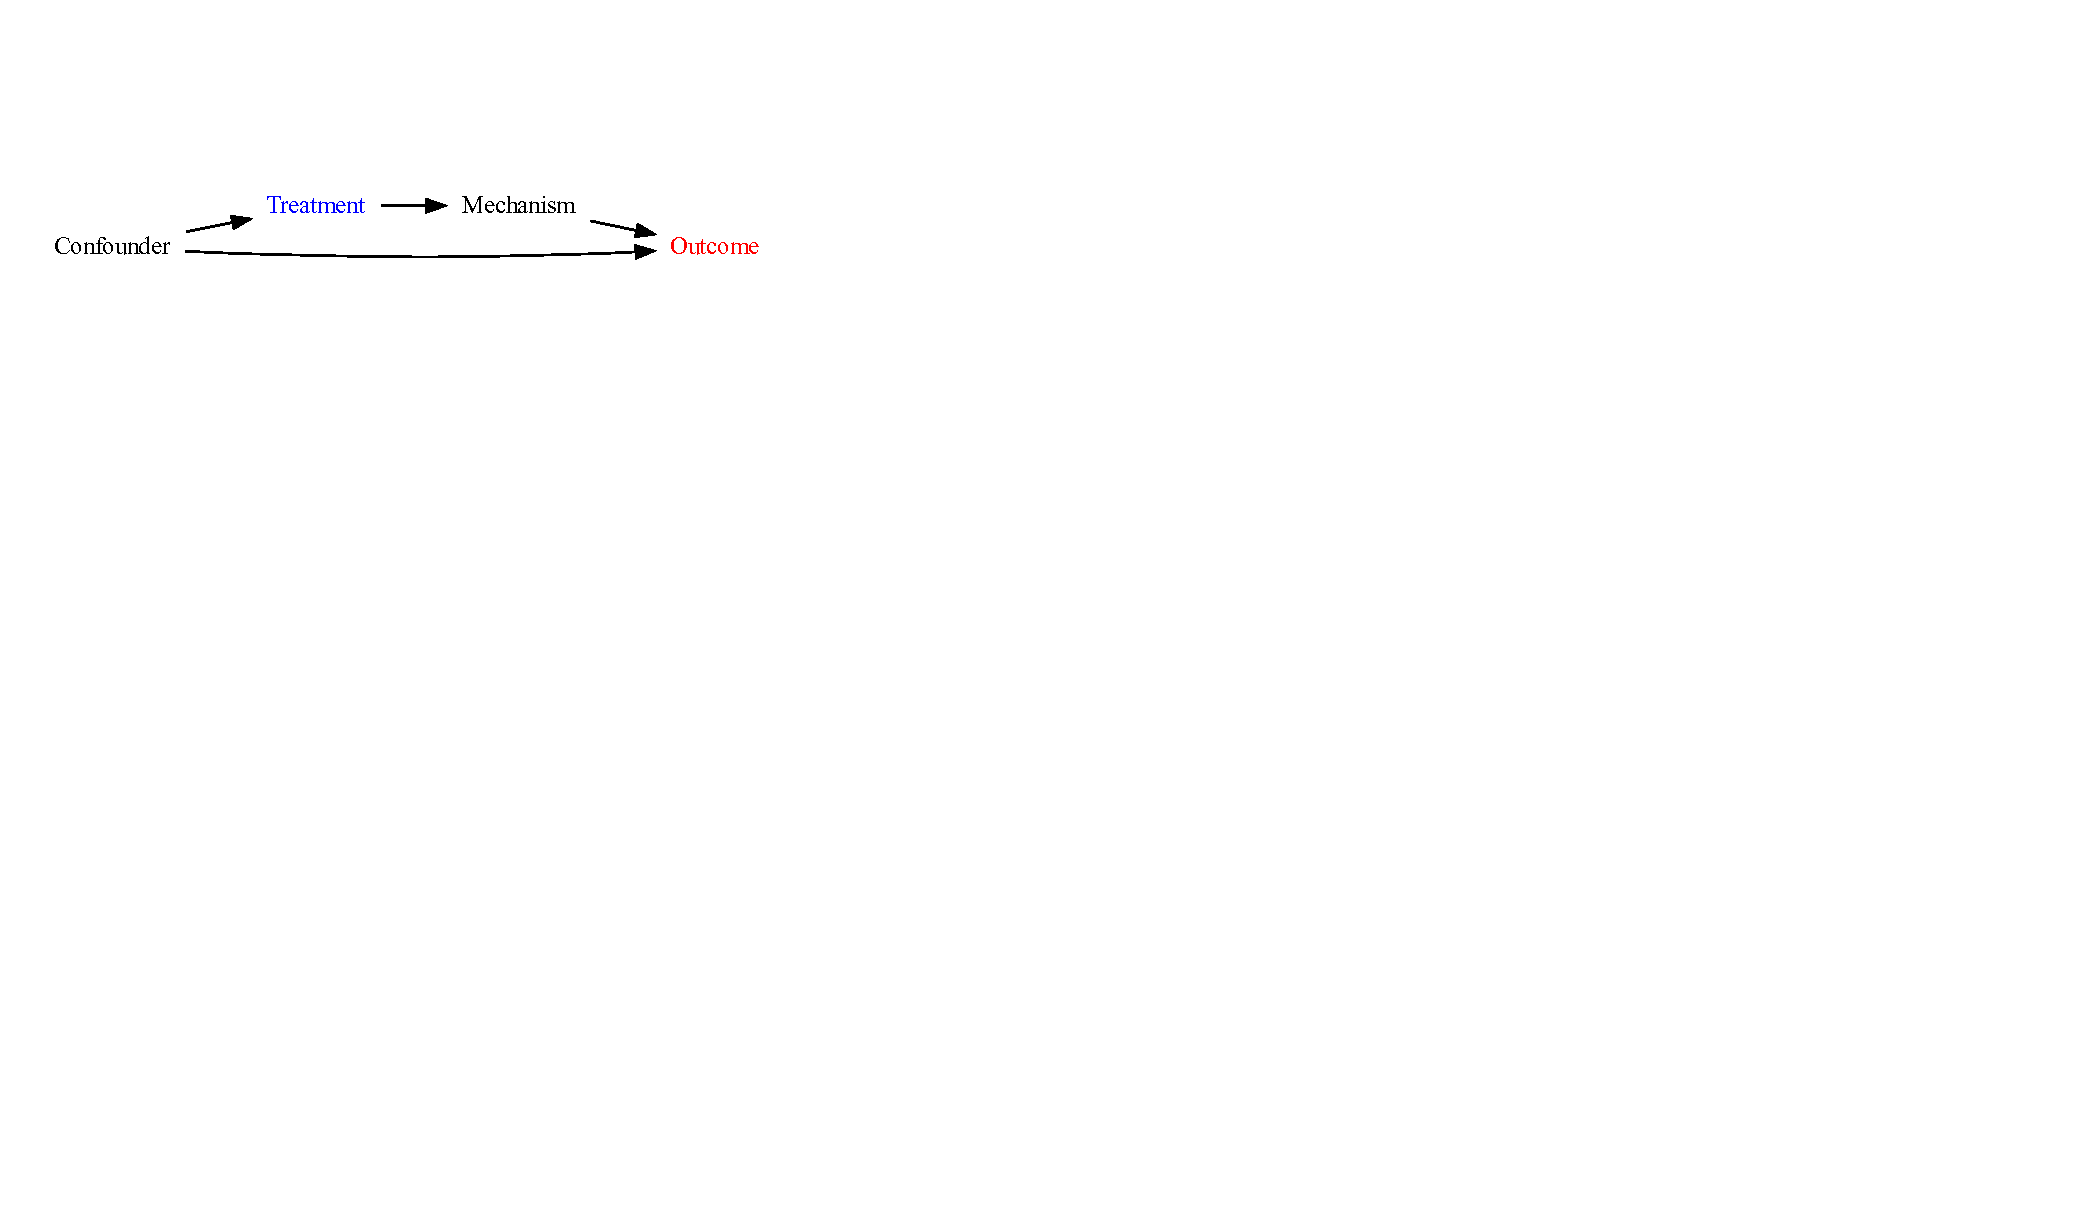
\includegraphics[width=1.8\linewidth]{figure/Dag3b-1} 

\end{knitrout}
\end{frame}


\begin{frame}
\frametitle{Process Tracing}
\begin{itemize}
\item We can also test mechanisms on the causal path of confounders:
\pause
\begin{itemize}
\item Evidence of Mechanism X NOT occurring can rule out this alternative theory
\pause
\item Evidence of Mechanism X occurring is consistent with Treatment having a causal effect, but not proof
\pause
\end{itemize}
\item This is a 'straw in the wind' test
\end{itemize}
\begin{knitrout}
\definecolor{shadecolor}{rgb}{0.969, 0.969, 0.969}\color{fgcolor}
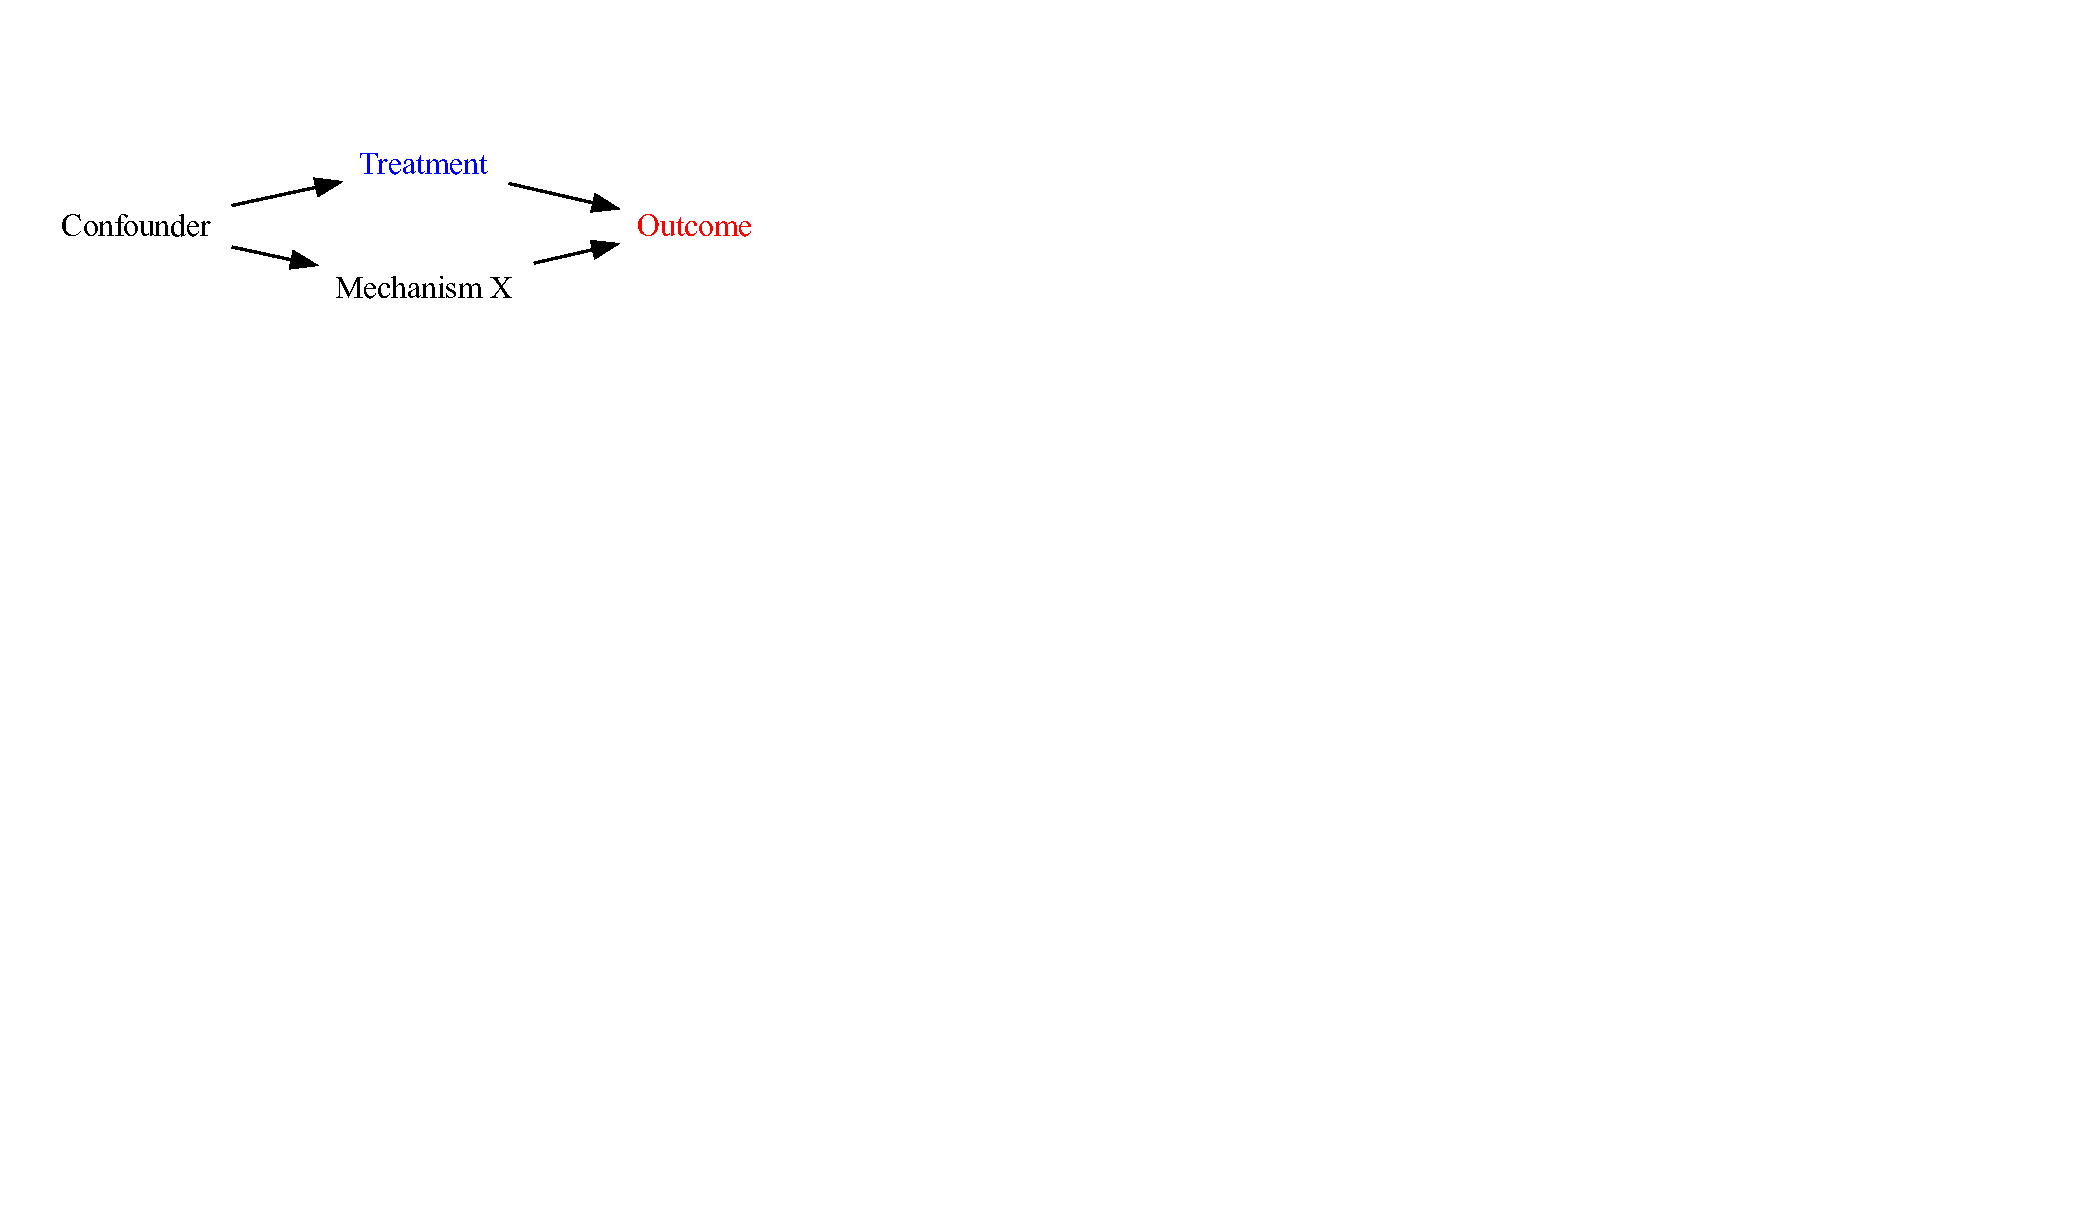
\includegraphics[width=1.8\linewidth]{figure/Dag4-1} 

\end{knitrout}
\end{frame}

\begin{frame}
\frametitle{Process Tracing}
\begin{itemize}
\item Unusually, a mechanism might explicitly separate two theories:
\pause
\begin{itemize}
\item $M=0$ if treatment is active
\pause
\item $M=1$ if the confounder is active
\pause
\end{itemize}
\item This is a 'Doubly-Decisive' test
\end{itemize}
\begin{knitrout}
\definecolor{shadecolor}{rgb}{0.969, 0.969, 0.969}\color{fgcolor}
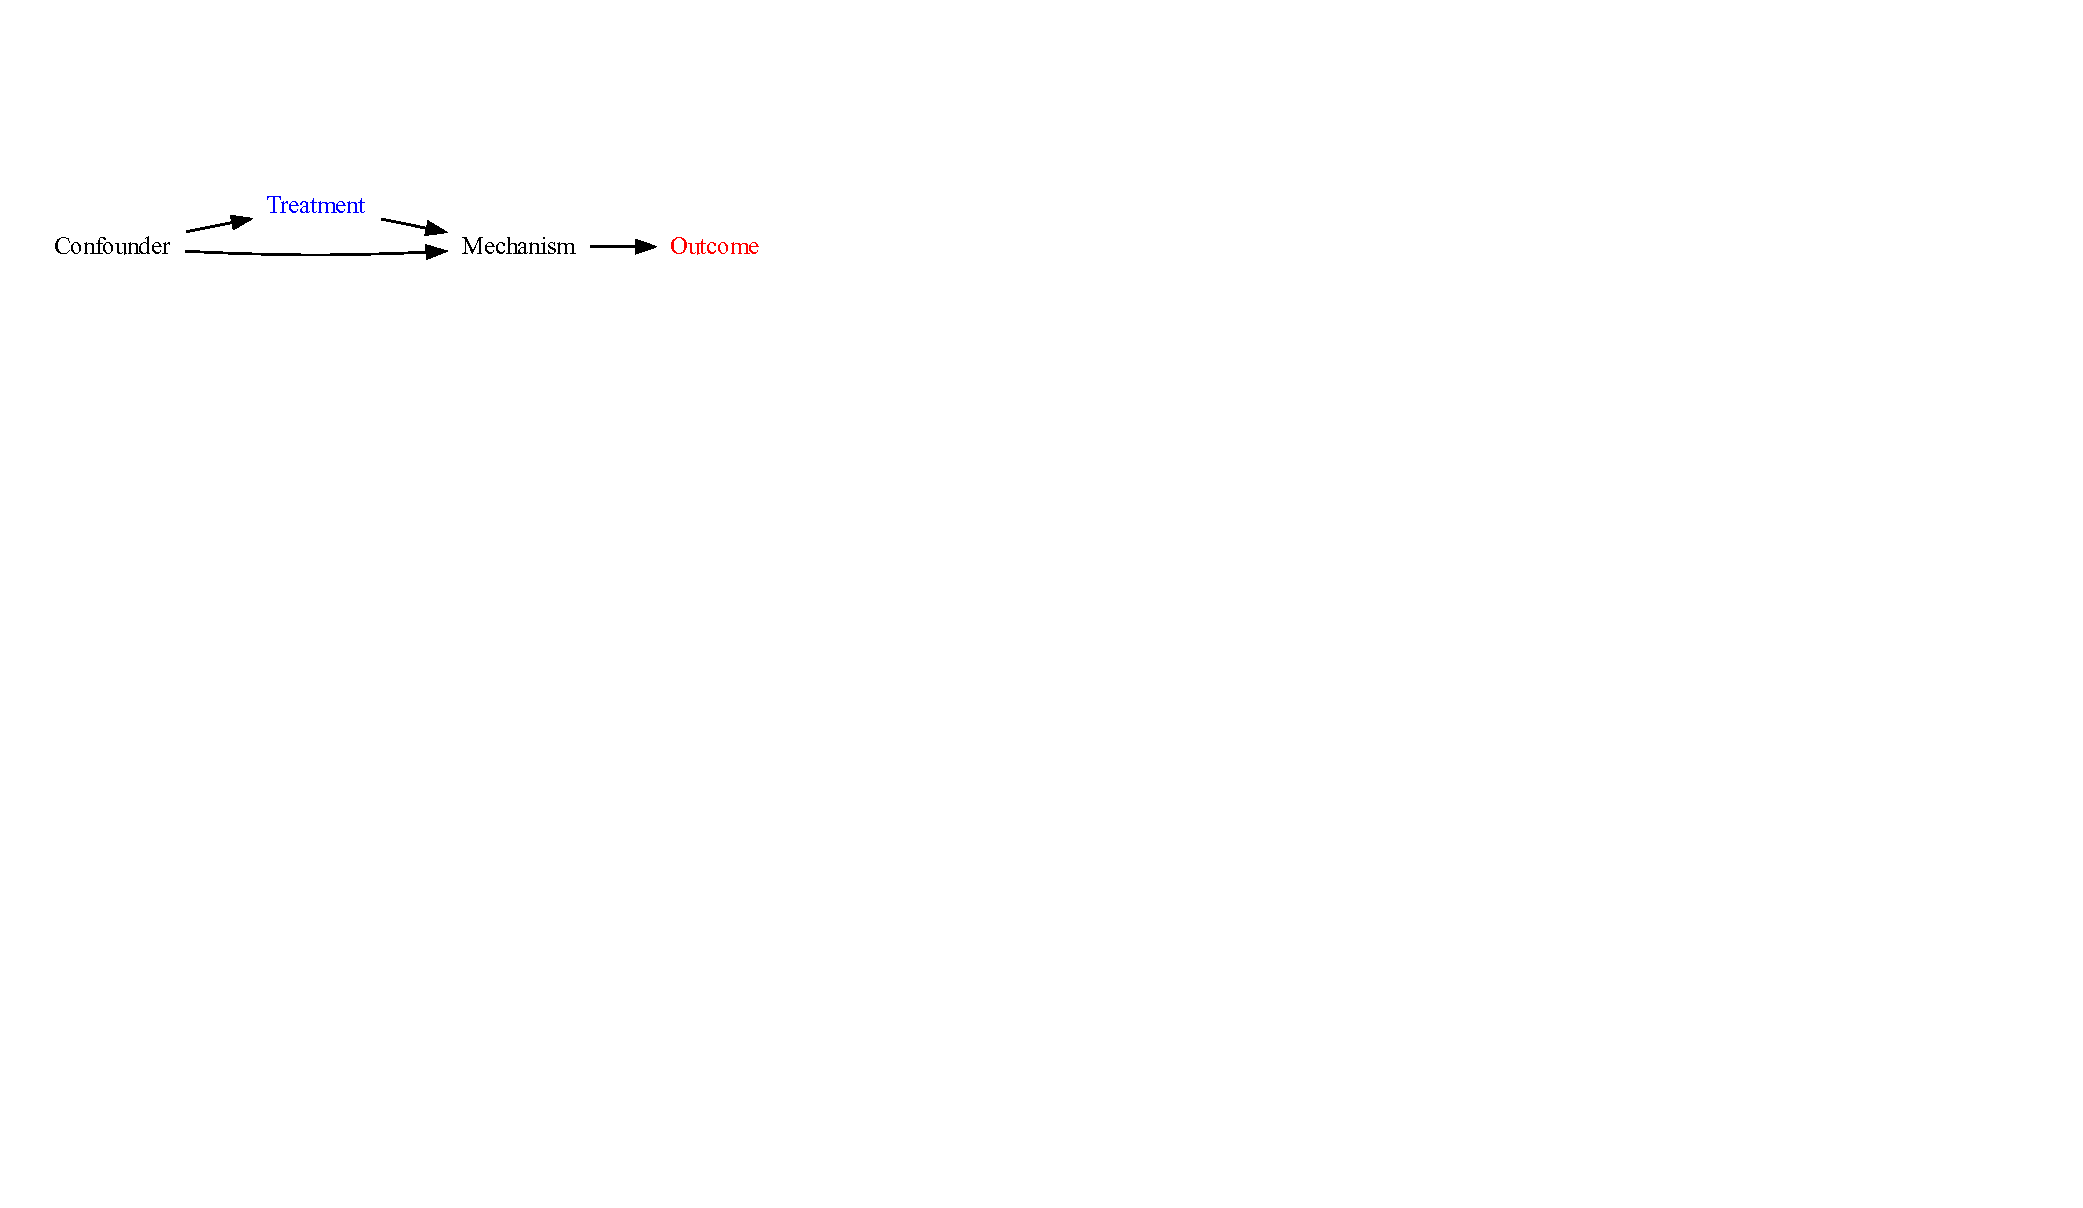
\includegraphics[width=1.8\linewidth]{figure/Dag5-1} 

\end{knitrout}
\end{frame}

\begin{frame}
\frametitle{Process Tracing}
\begin{itemize}
\footnotesize
\item Does Development cause Democracy?
\pause
\item We only have knowledge about South Korea: It got much richer between 1960 and 1987 when it became a democracy
\pause
\begin{multicols}{2}
\item But did higher income \textit{cause} democracy?
\pause
\item Higher incomes raise the demand for democracy, and diversify power away from the state
\pause
\item If this were true we should see:
\begin{itemize}
\item Opinion polls show increased support for democracy
\pause
\item Street protests, especially among the new middle-class
\pause
\item Private sector and civil society lobbying for democracy
\end{itemize}
\pause
\columnbreak
\item Or was it American pressure (alternative theory)?
\pause
\item South Korean elites faced costs to continuing dictatorship, and choose to democratize
\pause
\item If this were true we should see:
\begin{itemize}
\item Discussions (public or private) between US and Korean elites
\pause
\item Korean vulnerability to US pressure
\pause
\item Elites choosing the time and form of democratization
\end{itemize}
\end{multicols}
\end{itemize}
\normalsize
\end{frame}

\begin{frame}
\frametitle{Process Tracing}
\begin{itemize}
\item What does the evidence show?
\pause
\vspace{2cm}
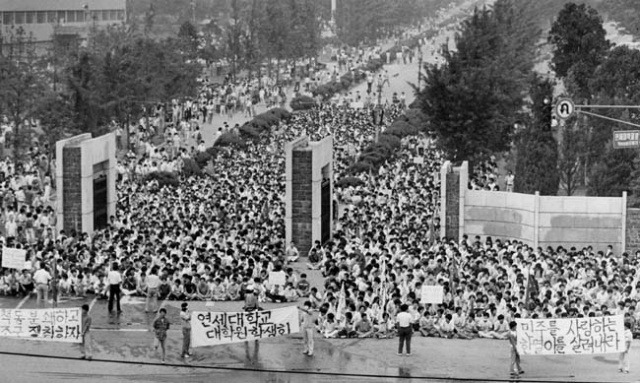
\includegraphics[width=0.9\linewidth]{South_Korea.jpg}
\end{itemize}
\end{frame}

\begin{frame}
\frametitle{Process Tracing}
\begin{itemize}
\item What happened to counterfactuals here?
\pause
\item We still don't know what would have happened if our case had not received the treatment
\pause
\item We're substituting assumptions/theory for a counterfactual
\pause
\begin{itemize}
\item We 'assume' that the only way our treatment could work is through the mechanism we specify
\pause
\item And we assume the only way confounding works is through the mechanism we specify
\end{itemize}
\item So everything depends on how confident we are in our theory/assumptions about mechanisms
\end{itemize}
\end{frame}

\begin{frame}
\frametitle{Process Tracing}
\begin{itemize}
\item In practice, process tracing is made harder by:
\pause
\begin{itemize}
\item Imprecise, or non-discriminating theory
\pause
\item Imperfect measurement and data availability
\pause
\item Subjective judgment on the weight of each piece of evidence
\end{itemize}
\end{itemize}
\end{frame}

\begin{frame}
\frametitle{Process Tracing}
\begin{itemize}
\item What are we really learning from process tracing?
\pause
\item That a treatment caused an outcome \textbf{in our specific case}
\pause
\item But how representative is our case?
\pause
\item Will the same causal effect occur in other contexts?
\end{itemize}
\end{frame}

%Framework relies on deterministic effects, not probabilistic ones (really means we've taken all the confounders into account)

\begin{frame}
\frametitle{Process Tracing}
\begin{itemize}
\item Brady (2010)
\pause
\item Difference-in-differences evidence that the early announcement of a Democrat victory in Florida led to reduced Republican voting
\pause
\item Estimated 10,000 lost Republican votes
\pause
\item The only way the causal effect is true is if there is a causal mechanism connecting the treatment to the outcome:
\pause
\begin{itemize}
\item How long was left for the election after treatment?: \pause 10 minutes
\pause
\item How many voters were \textbf{potentially influenced}: \pause 4,200 voters
\pause
\item How many voters were \textbf{probably treated}: \pause 560 voters
\pause
\item How many voters \textbf{likely complied with treatment}: \pause 56 voters \pause < 10,000
\end{itemize}
\end{itemize}
\end{frame}

\end{document}
